%----------------------------------------------------------------------------
\chapter{Validáció}
\label{chp:validation}
%----------------------------------------------------------------------------

Ebben a fejezetben az alkalmazás tesztelési módját írom le, majd az éles környezetben elvégzett méréseket, amelyekkel különbőző teljesítményparamétereit elemzem, illetve hasonlítom össze a most használt terítési megoldásival.

%----------------------------------------------------------------------------
\section{Tesztelés}
%----------------------------------------------------------------------------

Az alkalmazás helyes működésének ellenőrzéséhez először funkcionális teszteket futtattam annak kisebb egységein a JUnit\cite{massol2003junit} keretrendszert használva. Mivel a program build-elése Maven-nel\cite{smart2005introduction} történik, minden új programverzió tesztelését automatizáltan el tudtam végezni, ráadásul a következő Maven-plugin-eket használva egyéb fontos tulajdonságait vizsgáltam meg a programnak:

\begin{itemize}
  \item PMD, Findbugs\cite{rutar2004comparison}: Mindkettő forráskód analízisét végzi, alapvető, de nehezen észrevehető hibák megtalálásában nyújtanak nagy segítséget (például fel nem szabadított erőforrások)
  \item Checkstyle\cite{checkstyle}: Kódminőség ellenőrzésére való, segítségével a kész termék forráskódját jó minőségűvé, más programozók által könnyen megérthetővé tehetjük.
\end{itemize}

A program integrációs tesztelését az éles laborkörnyezetben végeztem, ennek során születtek meg \aref{performanceanal}-es fejezet mérési eredményei is.

%----------------------------------------------------------------------------
\section{Teljesítményelemzés}
%----------------------------------------------------------------------------
\label{performanceanal}

A programom teljesítményének elemzése során különböző, az alkalmazás teljesítményével kapcsolatos, általam felvetett kérdésre próbálok választ adni. A mérések során különböző méretű (1, 2, 4, 8 GB) fájlok terítését fogom töbször elvégezni.

%
\subsection{Chaincast és Torrent alapú terítés idejének összehasonlítása}
%
\textbf{Kérdés:} Gyorsabb-e a Torrent alapú terítés a Chaincast-osnál?

\textbf{Mérés:} A kérdés megválaszolásához 1, 2, 4 és 8 GB méretű fájlokat terítettem az eredeti és az általam készített új terítési módszerrel, a mérés eredményeit  \aref{fig:chaincasttorrrentcomparison}-es~ábrán látható grafikon mutatja be.


\textit{Érdemes megjegyezni, hogy a grafikonon két időérték szerepel a Torrent-es terítéshez: egyik tartalmaza a torrent fájl elkészítésének és betöltésekor ennek hash-ellenőrzésének az idejét, míg a másik csak a konkrét adatátvitelét. Ez az időveszteség a bemenet méretétől függően nő, viszont nem lineárisan, ezért nagyon indokolt lenne a torrentklienset rákényszeríteni ennek a hash-ellenőrzésnek a kihagyására, főleg mivel ennek gyakorlati haszna nincs is.}

\textbf{Válasz:} Nem gyorsabb a Torrent alapú terítési megoldás, körülbelül kétszer lassúbb. Kijelenthető, hogy ez egy elfogadható kompromisszum a robusztusság javítása érdekében, főleg úgy, hogy az ábra nem tartalmazza, hogy adott Chaincast-os terítéshez hány sikertelen próbálkozás tartozik és ez mennyi időveszteséggel jár. 

\begin{figure}[ht]
\centering
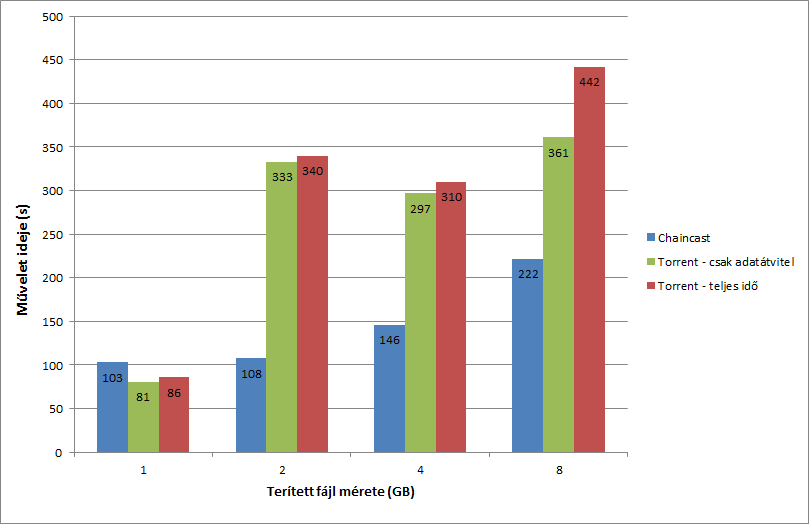
\includegraphics[width=150mm, keepaspectratio]{figures/Perf_chaincast_torrent_comparison.png}
\caption{Chaincast és Torrent alapú terítés idejének összehasonlítása}
\label{fig:chaincasttorrrentcomparison}
\end{figure}

%
\subsection{Skálázódás - Torrent alapú terítés 10 és 25 gépere}
%

\textbf{Kérdés:} Hogyan skálázódik a Torrent alapú terítés, mennyit változik a terítés ideje, ha több gépre terítünk?


\textbf{Mérés:} A fájlok terítését 10 és 25 gépre végeztem el, a kapott terítési idpknek az összehasonlítását a következő táblázat tartalmazza:

\begin{center}
	\begin{tabular}{ |c|>{\centering\arraybackslash}m{2.5cm}|>{\centering\arraybackslash}m{2.5cm}|>{\centering\arraybackslash}m{2.5cm}|>{\centering\arraybackslash}m{2.5cm}| }
		\hline
		\multirow{2}{*}{Fájlméret}&\multicolumn{2}{c|}{Terítés - teljes idő}&\multicolumn{2}{c|}{Terítés - csak az adatátvitel} \\
		& 10 gépre & 25 gépre & 10 gépre & 25 gépre \\
		\hline
		1 GB & 85 s & 86 s & 80 s & 81 s \\
		\hline
		2 GB & 178 s & 340 s & 167 s & 333 s \\
		\hline
		4 GB & 293 s & 310 s & 270 s & 297 s \\
		\hline
		8 GB & 563 s & 442 s & 516 s & 361 s \\
		\hline
	\end{tabular}
\end{center}

\textbf{Válasz:} Kisebb fájlok esetén kedvezőbb eredményt kaptunk a 10 gépes terítésre, viszont a terítendő fájl(ok) méretének növelésével a 25 gépes terítés jobban skálázódik. Összegezve, a kevesebb gépre végzett terítéshez képest legrosszabb esetben 1.9-szer rosszabb, a legjobb esetben 1.3-szor jobb eredményt kaptunk.

%
\subsection{P2P alapú fájlterítés - hibatűrés}
%
\textbf{Kérdés:} Hibatűrő-e a Torrent alapú fájterítési megoldás?

\textbf{Mérések:} A hibatűrési tesztet két részben végeztem el, az első részben azt néztem meg, hogy az én megoldásom hogyan reagál, ha a terítés indításakor van nem elérhető célgép. Ez Chaincast esetében automatikus bukást okoz, mivel ott küldés előtt ellenőrződik a teljes lánc létrejötte, és hiányzó gép esetében el sem kezdődik a fájlátvitel. Indítottam tehát egy terítést, ahol az egyik célgép nem volt bekapcsolva. A második teszt folyamán a fájlátvitel közben tettem gépeket elérhetetlenné, egyet kikapcsoltam, egynek megszűntettem a hálózati kapcsolatát, egyen pedig a torrentklienset zártam be manuálisan.

\textbf{Válasz:} Az új terítési megoldás hibatűrő, mivel az első teszt során a bekapcsolva hagyott összes gépre sikeresen terültek a fájlok, illetve a második teszt során az érintetlenül hagyott gépekre szintén. Továbbá a három kiesett gép a letöltést később folytatni tudta és azt be is fejezte.


%
\subsection{P2P alapú fájlterítés - szűk keresztmetszetek}
%

\textbf{Kérdés:} Vannak-e a laborban olyan gépek, amelyekre az átlagnál jelentősen lassabban megy a Torrent alapú terítés?

\textbf{Mérés:} Az előző mérések elvégzése közben feljegyeztem, hogy melyik gépek fejezték be a letöltést leghamarabb és legkésőbb, \aref{fig:computerdownloadspeeds}-es ábra mutatja, hogy adott gép hányszor szerepelt a terítések végén a 3 leglassabb, illetve leggyorsabb gép között.

\begin{figure}[ht]
\centering
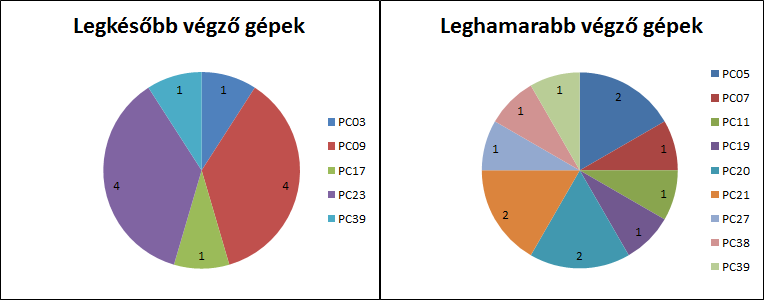
\includegraphics[width=150mm, keepaspectratio]{figures/Perf_computers.png}
\caption{Letöltést leghamarabb/legkésőbb befejező gépek}
\label{fig:computerdownloadspeeds}
\end{figure}

\textbf{Válasz:} Igen, vannak olyan gépeink, amelyekre lassabban megy a terítés, konkrétan a 23 és a 9-es sorszámúak. Mivel a másik véglet mérésénel nem voltak kiugró gyakoriságok, feltehetjük, hogy ezekkel a gépekkel kapcsolatos kijavítandó problémát állnak fenn (például merevlemez cseréje vagy a géphez kapcsolódó hálózati eszköz cseréje).


